\documentclass[12pt]{article}

% Margins
\usepackage[letterpaper, top=1in, bottom=1in, left=1in, right=1in]{geometry}

% Text over arrows
\usepackage{mathtools}

% Graphics and subcaptions
\usepackage{graphicx}
\usepackage{float}

% For code
\usepackage{courier}
\usepackage{listings}
\lstset{ mathescape }
\lstset{basicstyle=\ttfamily\footnotesize,breaklines=true}

% Remove Default sections headers
\setcounter{secnumdepth}{0}

% Clickable Table of Contents
\usepackage{color}   %May be necessary if you want to color links
\usepackage{hyperref}
\hypersetup{
	colorlinks=true, %set true if you want colored links
	linktoc=all,     %set to all if you want both sections and subsections linked
	linkcolor=black,  %choose some color if you want links to stand out
}

% Change Font
\usepackage[sfdefault]{roboto}  %% Option 'sfdefault' only if the base font of the document is to be sans serif
\usepackage[T1]{fontenc}


\usepackage[english]{babel}
\usepackage[utf8]{inputenc}
\usepackage{fancyhdr}

% For double spacing
\usepackage{setspace}

\usepackage[english]{babel}
\usepackage[utf8]{inputenc}
\usepackage{fancyhdr}

\pagenumbering{arabic}

\pagestyle{fancy}
\rhead{Hickey, Kovach, Saunders, Stewart}

\lhead{ST 501 R Project}

% Add \tab command
\newcommand\tab[1][1cm]{\hspace*{#1}}

% Add \mean bar command
\newcommand*\mean[1]{\bar{#1}}

%opening
\title{ST 501 R Project}
\author{Jimmy Hickey, Shaleni Kovach, Meredith Saunders, Stephanie Stewart}



\begin{document}
\maketitle
\tableofcontents
\clearpage

\doublespacing

\section{Part I - Convergence in Probability}

\subsection{1.}
Consider the "double exponential" or Laplace Distribution. A RV $Y \sim Laplace(\mu, b)$ has the PDF given by

$$f_Y(y) = \frac{1}{2b}e^{-\Big(  \frac{|y-\mu |}{b}   \Big) } $$

for $-\infty < y < \infty$, $-\infty < \mu < \infty$, and $b>0.$

We will consider having a random sample of Laplace RVs with $\mu = 0$ and $b = 5$. We'll look at the limiting behavior of $L=\frac{1}{n}\sum_{i=1}^{n}Y_i^2$ using simulation.

\subsubsection{a.}
Give a derivation of what $L$ converges to in probability. You should show any moment calculations and state the theorem(s) you use.

\bigskip


By the Weak Law of Large Numbers, we know that,

$$L = \frac{1}{n}\sum_{i=1}^{n}Y_i^2 \xrightarrow{\text{p}} E(Y^2).$$

We can calculate  $E(Y^2)$ using the definition of an expected value.

\begin{align*}
	 E(Y^2) & = \int_{-\infty}^{\infty} y^2 \cdot \frac{1}{2b} \cdot e^{-\Big(  \frac{|y-\mu |}{b} \Big)} dy\\
	 & =  \int_{-\infty}^{\infty} (x + \mu)^2 \cdot \frac{1}{2b} \cdot e^{-  \frac{|x|}{b}} dx & \text{taking } x = y - \mu\\
	 & = \frac{ 1 }{2b } \int_{-\infty}^{\infty} (x^2 + 2 \mu x  + \mu^2) \cdot e^{-  \frac{|x|}{b}}dx\\
	 & = \frac{ 1 }{2b } \Big[ \int_{-\infty}^{\infty} x^2 \cdot e^{-  \frac{|x|}{b}}dx+ \int_{-\infty}^{\infty} 2\mu x \cdot e^{-  \frac{|x|}{b}}dx+ \int_{-\infty}^{\infty} \mu^2 e^{-  \frac{|x|}{b}}dx \Big]\\
	 & = \frac{ 1 }{ 2b }[4b^3 + 0 + 2b\mu^2]\\
	 & = \frac{ 4b^3 }{ 2b } + \frac{ 2b\mu^2 }{ 2b }\\
	 & = 2b^2 + \mu
\end{align*}

We can confirm this by checking $ E(Y)^2 = Var(Y) + E(Y)^2$. From Wikipedia, we can see that $E(Y) = \mu$ and $Var(Y) = 2b^2$.

$$Var(Y) + E(Y)^2 = 2b^2 + (\mu)^2 = 2b^2 + \mu^2 = E(Y)^2$$

In the case of $\mu =0, \ b = 5$, we get that $L \xrightarrow{\text{p}} 2\cdot 5^2 + 0 = 50$.

\subsubsection{b.}
Explain what $K = \sqrt{L}$ converges to and why.

\bigskip

By the Continuity Theorem, we can see that $K = \sqrt{L}  \xrightarrow{\text{p}}  \sqrt{2b^2 +\mu^2}$. In the case of $\mu =0, \ b = 5$, we get that $K \xrightarrow{\text{p}}  \sqrt{50}$.

\subsubsection{c.}
Derive the CDF of $Y$ . Note you’ll have two cases and you should show your work.

\bigskip
Our CDF looks like
$$F_Y(y) = \int_{-\infty}^{y}\frac{1}{2b}e^{-\Big(  \frac{|x-\mu |}{b}   \Big) }  dx$$

Using the absolute value, we can split the density function into two pieces, $y< \mu$ and $y\geq \mu$. Let us examine the first case.

\begin{align*}
F_Y(y) & = \int_{\infty}^{y} \frac{1}{2b}e^{-\frac{\mu-x}{b} } dx & \text{for } y <\mu\\
	& =  \int_{\infty}^{y} \frac{1}{2b}e^{\frac{x-\mu}{b} } dx \\
	& = \frac{1}{2} e^{\frac{y-\mu }{b}}
\end{align*}

Next we can examine the $y\geq \mu$ case.

\begin{align*}
F_Y(y) & = \int_{\infty}^{y} \frac{1}{2b}e^{-\frac{x - \mu}{b} } dx & \text{for } y \geq\mu\\
& =  \int_{\infty}^{\mu} \frac{1}{2b}e^{\frac{\mu - x}{b} } dx + \int_{\mu}^{y} \frac{1}{2b}e^{\frac{\mu - x}{b} } dx  \\
& = \frac{ 1}{ 2 } + \Big(\frac{ 1}{ 2 } - \frac{ 1 }{ 2 } e^{\frac{ \mu - y }{ b }}\Big) \\
& = 1 - \frac{ 1 }{ 2 } e^{\frac{ \mu - y }{ b }}
\end{align*}

Putting the pieces together gives,

$$F_Y(y) = \begin{cases}
 \frac{1}{2} e^{\frac{y-\mu }{b}} & \text{for } y <\mu \\
1 - \frac{ 1 }{ 2 } e^{\frac{ \mu - y }{ b }} &  \text{for } y \geq\mu.
\end{cases}$$

\subsubsection{d. \& e.}

The code for parts d. and e. can be found in the \lstinline{Problem_1.R} file. Here are the resulting graphs.



\begin{figure}[H]
	\centering
	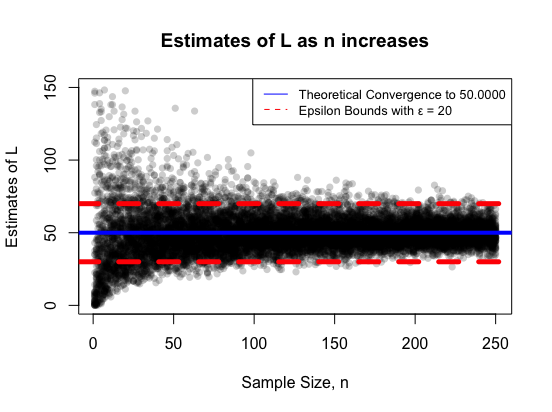
\includegraphics{img/n_vs_Ln.png}
	\caption{$L$ as $n$ increases}
\end{figure}

\begin{figure}[H]
	\centering
	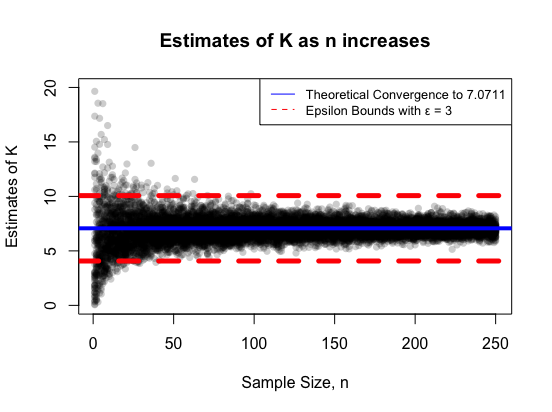
\includegraphics{img/n_vs_Kn.png}
	\caption{$K$ as $n$ increases}
\end{figure}

These graphs both demonstrate that our RVs $L$ and $K$ are converging in probability At each sample size $n$, the same number of samples ($50$) were taken.  Notice the trend as the number of observations ($n$) in each sample increases. It is clear that there is far less spread. As n increases, the RVs are converging to the blue line. The observed values of $L$ are geting closer and closer to $50$. And the observed values of $K$ are approaching $\sqrt{50}$.  As $n$ increases we could continue to shrink our epsilon bubble around the expected value and we will continue to see this convergence.


\section{Part II - Convergence in Distribution}

\subsection{2.}
This time we’ll look at the limiting distribution of our statistics.

\subsection{3.}
Theoretically, since $L$ is an average of \textit{iid} RVs ($Y_i^2$ß are each RVs) with finite variance
we know that, properly standardized, $L$ should have a standard normal limiting distribution by the CLT. 

Derive the appropriate standardization that will converge to a standard normal distribution for $\mu = 0$ and an arbitrary $b$. Show your work. Note: the kurtosis of the
Laplace distribution is 6 and we have $\mu = 0$. Find the formula for kurtosis (book or
wikipedia) and the calculation of the fourth moment won’t be too bad!

\subsection{4.}
Redo your above 4 plots using the standardization.

The graphs were generated using the standardization of $L$, along with the value of $b$ that was provided in part I. Each graph shows to have a similar shape that is approaching a normal distribution. Further increasing the size of $n$, would continue to show the distribution converging to a normal distribution. 

\begin{figure}[H]
	\centering
	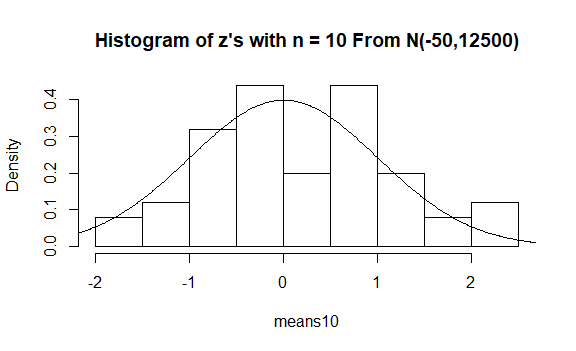
\includegraphics{img/Rplot_4a.png}
	\caption{50 samples at $n=10$}
\end{figure}

\begin{figure}[H]
	\centering
	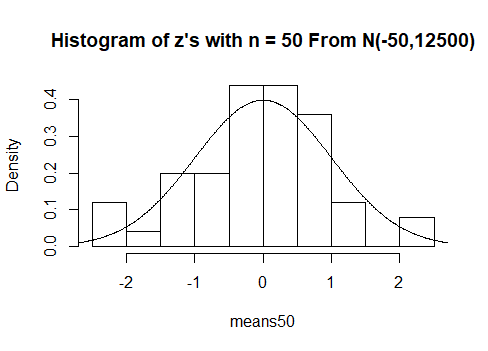
\includegraphics{img/Rplot_4b.png}
	\caption{50 samples at $n=50$}
\end{figure}

\begin{figure}[H]
	\centering
	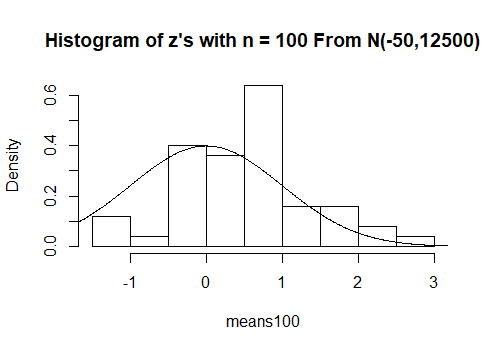
\includegraphics{img/Rplot_4c.png}
	\caption{50 samples at $n=100$}
\end{figure}

\begin{figure}[H]
	\centering
	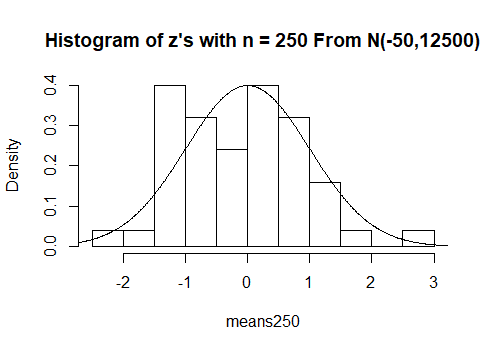
\includegraphics{img/Rplot_4d.png}
	\caption{50 samples at $n=250$}
\end{figure}



\subsection{5. \& 6.}
 Now let’s see if convergence is occurring for larger values of $n$. Generate data using the
same method as above except do so for $n = 1000$ and $n = 10,000$. Use $N = 10,000$
data sets as well.
Create similar plots for these two n values. In a comment discuss how the CLT is
manifesting for this problem. Does n > 30 work?

Using $N=50$, while the samples seem to be converging to normal, they still do not appear quite normal even for sample size $n=10,000$.
When we change to $N=10,000$ both $n=1,000$ and $n=10,000$ appear normal.
This shows it is not enough for $n>30$ the number of sample repetitions also plays a role in CLT..

\begin{figure}[H]
	\centering
	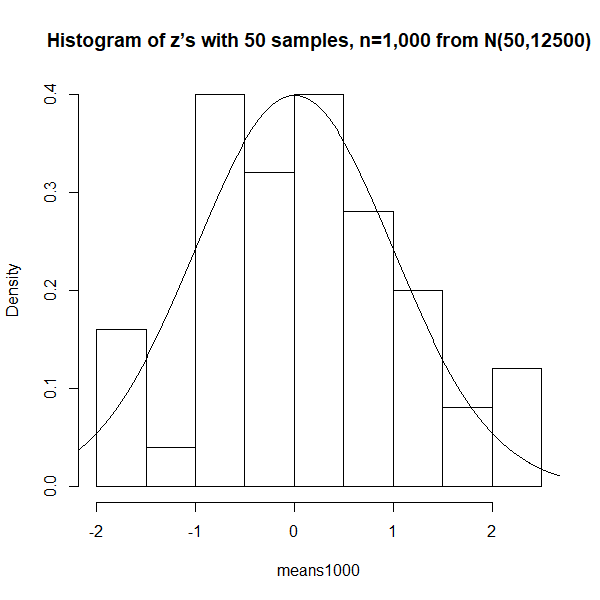
\includegraphics{img/Problem6_1.png}
	\caption{50 samples at $n = 1,000$}
\end{figure}

\begin{figure}[H]
	\centering
	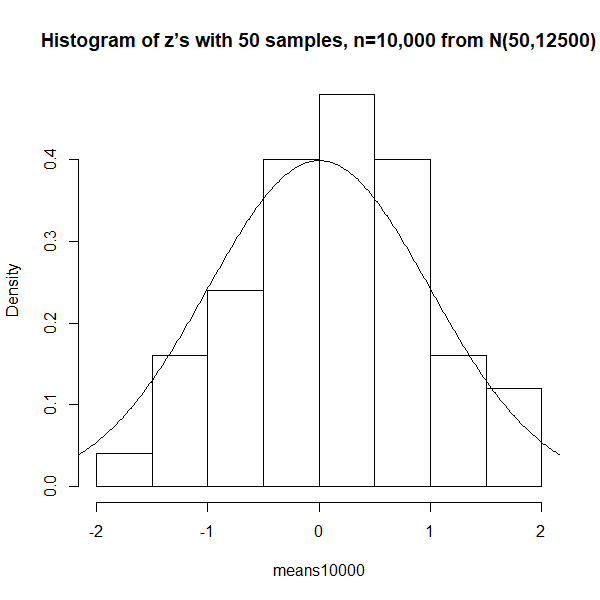
\includegraphics{img/Problem6_2.png}
	\caption{50 samples at $n=10,000$}
\end{figure}

\begin{figure}[H]
	\centering
	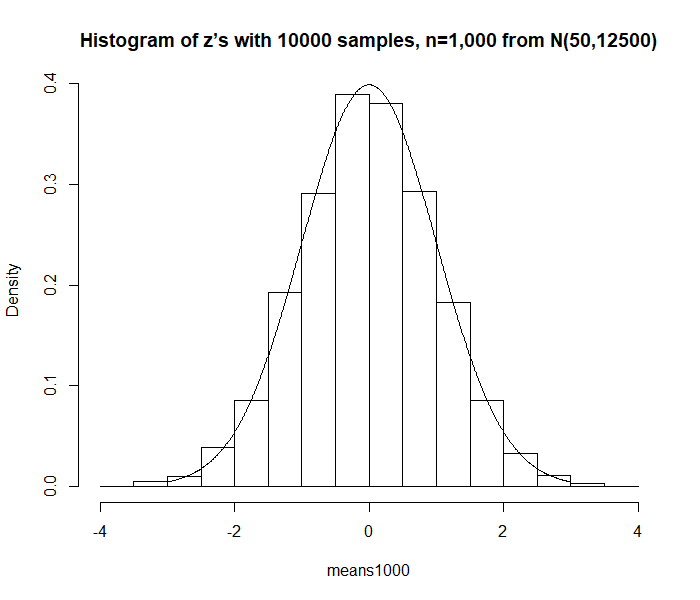
\includegraphics{img/Problem6_3.png}
	\caption{10,000 samples at $n=1,000$}
\end{figure}

\begin{figure}[H]
	\centering
	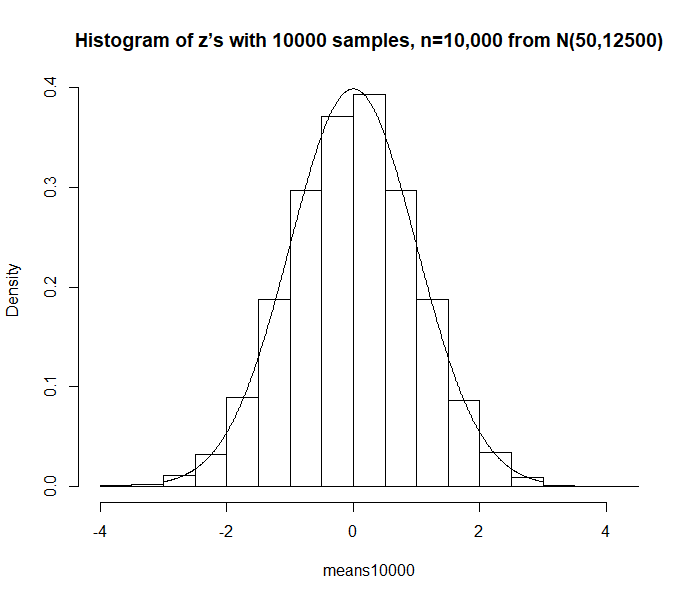
\includegraphics{img/Problem6_4.png}
	\caption{10,000 samples at $n=10,000$}
\end{figure}



\end{document}
